%%%%%%%%%%%%%%%%%%%%%%%%%%%%%%%%%%%%%%%%%
% Journal Article
% LaTeX Template
% Version 1.4 (15/5/16)
%
% This template has been downloaded from:
% http://www.LaTeXTemplates.com
%
% Original author:
% Frits Wenneker (http://www.howtotex.com) with extensive modifications by
% Vel (vel@LaTeXTemplates.com)
%
% License:
% CC BY-NC-SA 3.0 (http://creativecommons.org/licenses/by-nc-sa/3.0/)
%
%%%%%%%%%%%%%%%%%%%%%%%%%%%%%%%%%%%%%%%%%

%----------------------------------------------------------------------------------------
%	PACKAGES AND OTHER DOCUMENT CONFIGURATIONS
%----------------------------------------------------------------------------------------

\documentclass[twoside,twocolumn]{article}

\usepackage{blindtext} % Package to generate dummy text throughout this template 

\usepackage{hyperref}
\hypersetup{
    colorlinks=true,
    linkcolor=blue,
    filecolor=magenta,      
    urlcolor=cyan,
}

\usepackage[sc]{mathpazo} % Use the Palatino font
\usepackage[T1]{fontenc} % Use 8-bit encoding that has 256 glyphs
\linespread{1.05} % Line spacing - Palatino needs more space between lines
\usepackage{microtype} % Slightly tweak font spacing for aesthetics
\usepackage[utf8]{inputenc}

\usepackage[portuguese]{babel} % Language hyphenation and typographical rules

\usepackage[hmarginratio=1:1,top=32mm,columnsep=20pt]{geometry} % Document margins
\usepackage[hang, small,labelfont=bf,up,textfont=it,up]{caption} % Custom captions under/above floats in tables or figures
\usepackage{booktabs} % Horizontal rules in tables

\usepackage{lettrine} % The lettrine is the first enlarged letter at the beginning of the text
\usepackage{float}
\usepackage{enumitem} % Customized lists
\setlist[itemize]{noitemsep} % Make itemize lists more compact

\usepackage{abstract} % Allows abstract customization
\renewcommand{\abstractnamefont}{\normalfont\bfseries} % Set the "Abstract" text to bold
\renewcommand{\abstracttextfont}{\normalfont\small\itshape} % Set the abstract itself to small italic text
%\usepackage[shortlabels]{enumitem}
\usepackage{enumitem}
\usepackage{titlesec} % Allows customization of titles
\renewcommand\thesection{\Roman{section}} % Roman numerals for the sections
\renewcommand\thesubsection{\roman{subsection}} % roman numerals for subsections
\titleformat{\section}[block]{\large\scshape\centering}{\thesection.}{1em}{} % Change the look of the section titles
\titleformat{\subsection}[block]{\large}{\thesubsection.}{1em}{} % Change the look of the section titles

\usepackage{fancyhdr} % Headers and footers
\pagestyle{fancy} % All pages have headers and footers
\fancyhead{} % Blank out the default header
\fancyfoot{} % Blank out the default footer
\fancyhead[C]{MO443 $\bullet$ Maio 2019 $\bullet$ Relatório 03} % Custom header text
\fancyfoot[RO,LE]{\thepage} % Custom footer text

\usepackage{titling} % Customizing the title section

\usepackage{hyperref} % For hyperlinks in the PDF

\usepackage{graphicx}
\usepackage{subfigure}

\usepackage{mathtools}
\DeclarePairedDelimiter\floor{\lfloor}{\rfloor}
%----------------------------------------------------------------------------------------
%	TITLE SECTION
%----------------------------------------------------------------------------------------

\setlength{\droptitle}{-4\baselineskip} % Move the title up

\pretitle{\begin{center}\Huge\bfseries} % Article title formatting
\posttitle{\end{center}} % Article title closing formatting
\title{Relatório - Trabalho 03 \\ \Large MO443 - Introdução ao Processamento de Imagem Digital} %
%\subtitle{qsdqwdqwd} %Article title
\author{%
\textsc{Vinicius Teixeira de Melo - RA: 230223} \\[1ex] % Your name
\normalsize Universidade Estadual de Campinas \\ % Your institution
\normalsize \href{mailto:viniciusteixeira@liv.ic.unicamp.br}{viniciusteixeira@liv.ic.unicamp.br} % Your email address
%\and % Uncomment if 2 authors are required, duplicate these 4 lines if more
%\textsc{Jane Smith}\thanks{Corresponding author} \\[1ex] % Second author's name
%\normalsize University of Utah \\ % Second author's institution
%\normalsize \href{mailto:jane@smith.com}{jane@smith.com} % Second author's email address
}
\date{\today} % Leave empty to omit a date
\renewcommand{\maketitlehookd}{%
%\begin{abstract}
%\noindent \blindtext % Dummy abstract text - replace \blindtext with your abstract text
%\end{abstract}
}

%----------------------------------------------------------------------------------------

\begin{document}

% Print the title
\maketitle

%----------------------------------------------------------------------------------------
%	ARTICLE CONTENTS
%----------------------------------------------------------------------------------------

\section{Especificação do Problema}

O objetivo deste trabalho é aplicar operadores morfológicos para segmentar regiões compreendendo texto e
não texto em uma imagem de entrada.

Os seguintes passos devem ser realizados:

\begin{enumerate}
	\item dilatação da imagem original com um elemento estruturante de 1 pixel de altura e 100 pixels de largura;
	\item erosão da imagem resultante com o mesmo elemento estruturante do passo (1);
	\item dilatação da imagem original com um elemento estruturante de 200 pixels de altura e 1 pixel de largura;
	\item erosão da imagem resultante com o mesmo elemento estruturante do passo (3);
	\item aplicação da intersecção (AND) dos resultados dos passos (2) e (4);
	\item fechamento do resultado obtido no passo (5) com um elemento estruturante de 1 pixel de altura e 30
pixels de largura;
	\item aplicação de algoritmo para identificação de componentes conexos (ver programa fornecido) sobre o
resultado do passo (6);
	\item para cada retângulo envolvendo um objeto, calcule:
	\begin{enumerate}
		\item razão entre o número de pixels pretos e o número total de pixels (altura x largura);
		\item razão entre o número de transições verticais e horizontais branco para preto e o número total de pixels pretos;
	\end{enumerate}
	\item criação de uma regra para classificar cada componente conexo, de acordo com as medidas obtidas no
passo (8), como texto e não texto.
	\item aplicação de operadores morfológicos apropriados para segmentar cada linha do texto em blocos de palavras. Coloque um retângulo envolvendo cada palavra na imagem original. Calcule o número total de linhas de texto e de blocos de palavras na imagem.
\end{enumerate}

%------------------------------------------------

\section{Entrada de Dados}

O código fonte criado para a execução de todas as tarefas está no notebook \textbf{Trabalho 03.ipynb}. O código foi criado para aceitar imagens em preto e branco no formato PBM (\textit{Portable Bitmap}).

Para executar o notebook, basta iniciar o ambiente \textit{Jupyter Notebook}, abrir o notebook \textbf{Trabalho 03.ipynb} e executar as células em ordem. Todo o algoritmo foi implementado na linguagem Python na versão 3.6.

As imagen de entrada utilizada no teste do algoritmo foi retirada da página do prof. Hélio Pedrini: \href{http://www.ic.unicamp.br/~helio/imagens_morfologia/}{Imagens}. Na pasta \textbf{imgs/} está a imagem em preto e branco utilizada no teste: \textbf{bitmap.pbm}. As dimensões da imagen de entrada utilizada é 1374 x 2233.

\begin{figure}[H]
\begin{center}
	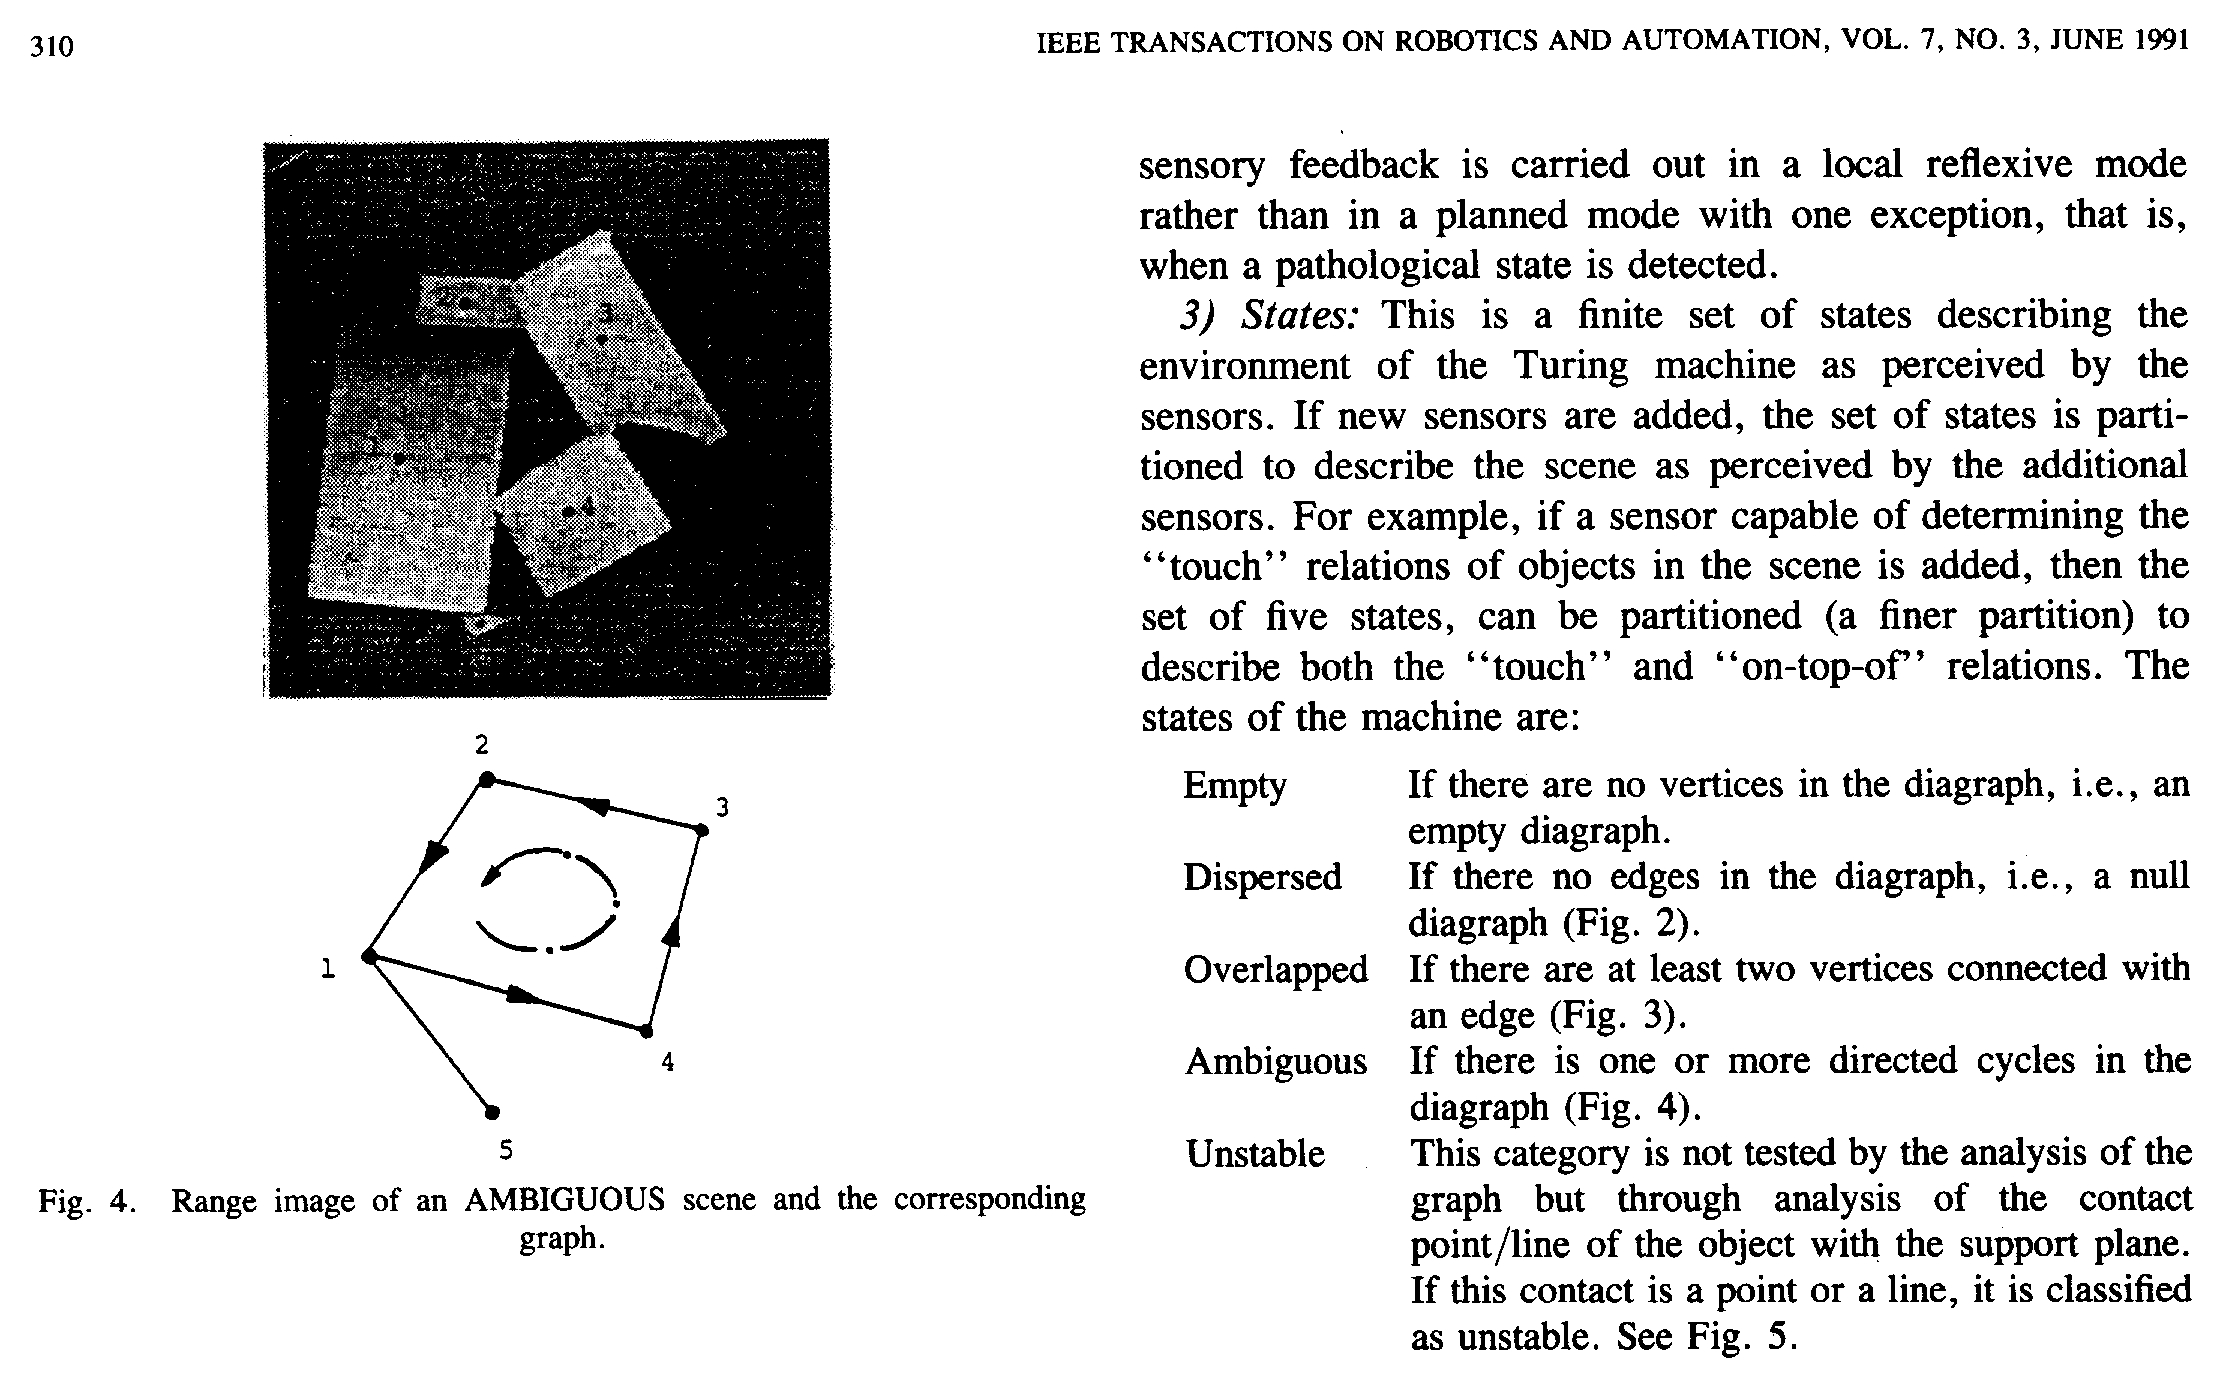
\includegraphics[height=4cm]{figures/bitmap.png}
\caption{bitmap.pbm} \label{gdimotes}
\end{center}
\end{figure}

%------------------------------------------------

\section{Dependências e Códigos}

As bibliotecas utilizadas neste trabalho foram:

\begin{table}[H]
\begin{tabular}{|l|l|}
\hline
\textbf{Biblioteca} & \textbf{Versão} \\ \hline
numpy               & 1.16.2          \\ \hline
cv2                 & 3.4.2           \\ \hline
matplotlib          & 3.0.3           \\ \hline
warnings            & 2.1             \\ \hline
\end{tabular}
\end{table}

A leitura das imagens foi realizada utilizando uma função do \textbf{opencv} \cite{b1} chamada \textbf{imread()}, a qual necessitou de uma constante do próprio \textbf{opencv} para que a imagem ficassem apenas com o canal de escala de cinza, essa constante é denominada \textbf{IMREAD\_GRAYSCALE}.

Os elementos estruturantes foram criados manualmente através da função \textbf{np.ones((\textit{shape}),np.uint8)}. Primeiramente, a imagem de entrada foi transformada para que as áreas de interesse estivessem com valor $255$. Para as operações de \textit{bits}, foram utilizadas as funções \textbf{cv2.bitwise\_not} e \textbf{cv2.bitwise\_and}.

Nas operações fundamentais de morfologia foram utilizadas com base nas funções \textbf{cv2.dilate} e \textbf{cv2.erose}. Para a operação de fechamento, foi utilizada a função \textbf{cv2.morphologyEx} com a constante do próprio OpenCv, chamada \textbf{cv2.MORPH\_CLOSE}.

No passo (7), para a detecção de componentes e criação dos \textit{bounding boxes} foi utilizada a função \textbf{cv2.findContours}, juntamente com as constantes \textbf{cv2.RETR\_TREE} e \textbf{cv2.CHAIN\_APPROX\_SIMPLE}. Assim, após a obtenção dos \textit{bounding boxes}, foram utilizadas as funções \textbf{cv2.boundingRect}, \textbf{cv2.rectangle} e \textbf{cv2.drawContours} para desenhar os \textit{bounding boxes} na imagem de entrada.

No passo (9), a regra utilizada para classificar um \textit{bounding box} como texto ou não foi: dado o valor $x_{a}$ obtido no passo (8.a) e o valor $x_{b}$ obtido no passo (8.b) referentes ao mesmo \textit{bounding box}, se $|x_{a} - x_{b}| \leq 0.2$, esse \textit{bounding box} é classificado como texto, se não, é classificado como não texto.


%------------------------------------------------

\section{Fundamentação}


%------------------------------------------------

\section{Saída de Dados}


%------------------------------------------------

\section{Resultados e Discuções}



%------------------------------------------------

\section{Conclusão}



%----------------------------------------------------------------------------------------
%	REFERENCE LIST
%----------------------------------------------------------------------------------------

\begin{thebibliography}{99} % Bibliography - this is intentionally simple in this template

\bibitem{b1} Welcome to opencv documentation! \href{https://docs.opencv.org/2.4/index.html}{https://docs.opencv.org/2.4/index.html} Acesso em: 04/05/2019.

\bibitem{b2} Pedrini, Hélio, and William Robson Schwartz. Análise de imagens digitais: princípios, algoritmos e aplicações. Thomson Learning, 2008.

\bibitem{b3} Matplotlib Version 3.0.3 \href{https://matplotlib.org/contents.html}{https://matplotlib.org/contents.html} Acesso em: 04/05/2019.
 
\end{thebibliography}

%----------------------------------------------------------------------------------------

\end{document}
